% Options for packages loaded elsewhere
\PassOptionsToPackage{unicode}{hyperref}
\PassOptionsToPackage{hyphens}{url}
%
\documentclass[
  11pt,
  a4paper,
]{article}
\usepackage{lmodern}
\usepackage{amssymb,amsmath}
\usepackage{ifxetex,ifluatex}
\ifnum 0\ifxetex 1\fi\ifluatex 1\fi=0 % if pdftex
  \usepackage[T1]{fontenc}
  \usepackage[utf8]{inputenc}
  \usepackage{textcomp} % provide euro and other symbols
\else % if luatex or xetex
  \usepackage{unicode-math}
  \defaultfontfeatures{Scale=MatchLowercase}
  \defaultfontfeatures[\rmfamily]{Ligatures=TeX,Scale=1}
  \setmainfont[]{Lato}
\fi
% Use upquote if available, for straight quotes in verbatim environments
\IfFileExists{upquote.sty}{\usepackage{upquote}}{}
\IfFileExists{microtype.sty}{% use microtype if available
  \usepackage[]{microtype}
  \UseMicrotypeSet[protrusion]{basicmath} % disable protrusion for tt fonts
}{}
\usepackage{xcolor}
\IfFileExists{xurl.sty}{\usepackage{xurl}}{} % add URL line breaks if available
\IfFileExists{bookmark.sty}{\usepackage{bookmark}}{\usepackage{hyperref}}
\hypersetup{
  pdftitle={Modelling electroglottographic data with wavegrams and generalised additive mixed models},
  pdfauthor={Stefano Coretta},
  hidelinks,
  pdfcreator={LaTeX via pandoc}}
% \urlstyle{same} % disable monospaced font for URLs
\usepackage[margin=1in]{geometry}
\usepackage{graphicx,grffile}
\makeatletter
\def\maxwidth{\ifdim\Gin@nat@width>\linewidth\linewidth\else\Gin@nat@width\fi}
\def\maxheight{\ifdim\Gin@nat@height>\textheight\textheight\else\Gin@nat@height\fi}
\makeatother
% Scale images if necessary, so that they will not overflow the page
% margins by default, and it is still possible to overwrite the defaults
% using explicit options in \includegraphics[width, height, ...]{}
\setkeys{Gin}{width=\maxwidth,height=\maxheight,keepaspectratio}
% Set default figure placement to htbp
\setlength{\emergencystretch}{3em} % prevent overfull lines
\providecommand{\tightlist}{%
  \setlength{\itemsep}{0pt}\setlength{\parskip}{0pt}}
\setcounter{secnumdepth}{5}
\usepackage{cleveref}
\usepackage[]{natbib}
\bibliographystyle{unified}

\title{Modelling electroglottographic data with wavegrams and generalised
additive mixed models}
\author{Stefano Coretta}
\date{}

\usepackage[absolute]{textpos}

\begin{document}
\begin{textblock}{3}(0.2,0.2)
  \textcolor{lightgray}{v0.1.9000 (2019/04/30)}
\end{textblock}
\maketitle

\hypertarget{introduction}{%
\section{Introduction}\label{introduction}}

\begin{figure}
  \centering
  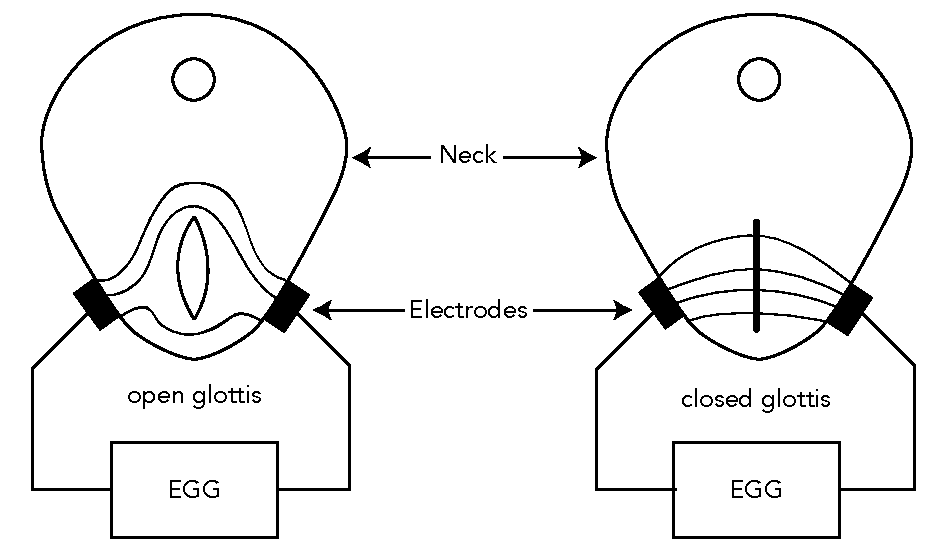
\includegraphics{./img/egg-setup.pdf}
  \caption{A schematics of the electroglottograph. A transverse section of the neck is shown with open glottis (on the left) and closed glottis (on the right). The electric field passing through the neck is represented by lines. When the vocal folds are apart, the opening distorts the electric field and impedance increases.}
  \label{f:egg-setup}
\end{figure}

The position of the vocal folds within the oral tract makes their
investigation difficult. Direct observation of the activity of the
larynx via invasive methods, like laryngeoscopy, brings with it a series
of practical drawbacks. Among other methods for obtaining information on
glottal activity is electroglottography. Electroglottography, or EGG
\citep{fabre1957}, is a technique that measures the degree of contact
between the vocal folds (the Vocal Folds Contact Area, VFCA). A high
frequency low voltage electrical current is sent through two electrodes
which are in contact with the surface of the neck, one on each side of
the thyroid cartilage (\Cref{f:egg-setup}). Impedance of this current is
modulated by the VFCA, and greater vocal folds contact creates less
impedance. The amplitude is inversely correlated with VFCA and
impedance, so that higher amplitude values indicate a greater contact
area \citep{titze1990}. The EGG unit registers the current impedance and
converts it to relative amplitude values. The time-developing amplitude
signal thus provides us with information on the changes in VFCA, i.e.~on
properties of vocal folds vibration (voicing).

\begin{figure}
  \centering
  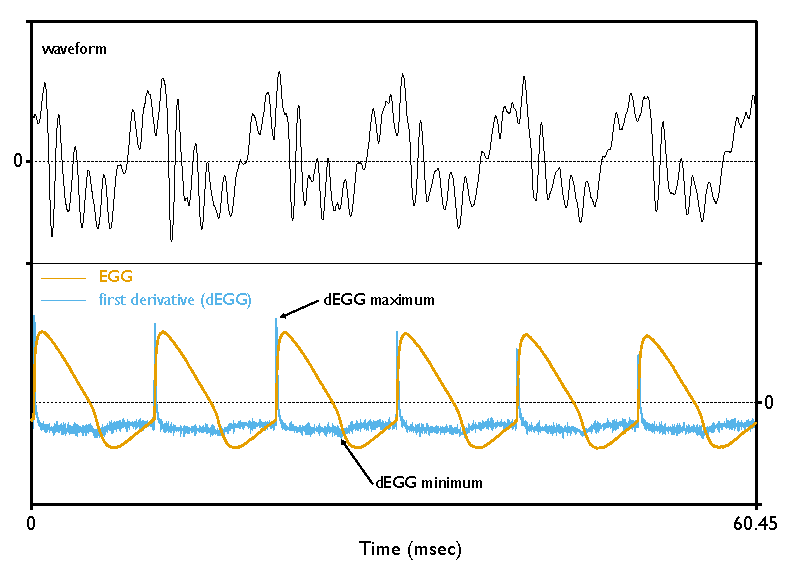
\includegraphics{./img/degg-signal.pdf}
  \caption{The electroglottographic signal (EGG) with corresponding first derivative (dEGG).}
  \label{f:egg}
\end{figure}

A glottal cycle can be described in terms of two phases
\citep{childers1985, hampala2016}: (a) a contacting phase, in which the
vocal folds are approaching each other, (b) a de-contacting phase, in
which the vocal folds move apart from each other. Transversal to this
two-phase description, the glottal cycle can be described in terms of
whether the glottis is closed or not. According to this classification,
the cycle can be divided into (1) a closed phase, in which the glottis
is completely closed and glottal flow is 0 (in some contexts this phase
could be absent, like in breathy voicing), and (2) an open phase, in
which there is no complete contact between the vocal folds. The timing
of these phases can be approximated from the EGG signal, as demonstrated
by both experimental and modelling work \citep{hampala2016}. An example
EGG signal is provided in \Cref{f:egg}.

Two important landmarks of glottal movement are the closing instant (the
timepoint of glottal complete closure) and the opening instant (the
moment in which the glottis first opens). These points delimit the open
and closed phases of a glottal cycle. The ratio of the closed phase
relative to the total cycle duration, the closed quotient, has been used
as an index of phonation type. Modal voice has higher close quotient
values than breathy voice, and lower values than creaky voice. One
method for the detection of the closing and opening instants is based on
the first derivative of the EGG signal (the dEGG, see \Cref{f:egg}).
\citet{herbst2017}, however, showed that this method returns values that
are just a surrogate of the actual articulatory movements, due to the
complex anatomy of the vocal folds, and that there are no clear
contacting and decontact instants, but rather intervals.
\citet{herbst2017} call this EGG-based closed quotient the `contact
quotient' and recommend to keep it distinct from the closed quotient
obtained from direct observation of the vocal folds.

As an alternative to the contact quotient, \citet{herbst2010} propose
the wavegram, a visualisation method which does not reduce the EGG
signal to a single value and thus suffers less from the limitations of
the contact quotient. The wavegram exploits information from the whole
signal to obtain an image of vocal folds activity. A wavegram is a 3D
representation of the EGG signal developing in time. Its structure is
similar to that of a classical phonetic spectrogram. The \emph{x}-axis
indicates the temporal sequence of individual glottal cycles. The
\emph{y}-axis represents the time within each glottal cycle, normalised
between 0 and 1. Finally, the normalised amplitude of the signal
corresponds to different colour intensities. Differences in intensity
along the \emph{x}-axis indicate changes in glottal activity. The
procedure for constructing a wavegram is given in \Cref{f:wavegram}. A
wavegram can be produced for the EGG signal and for any of its
transformations, like the dEGG.

\begin{figure}
  \centering
  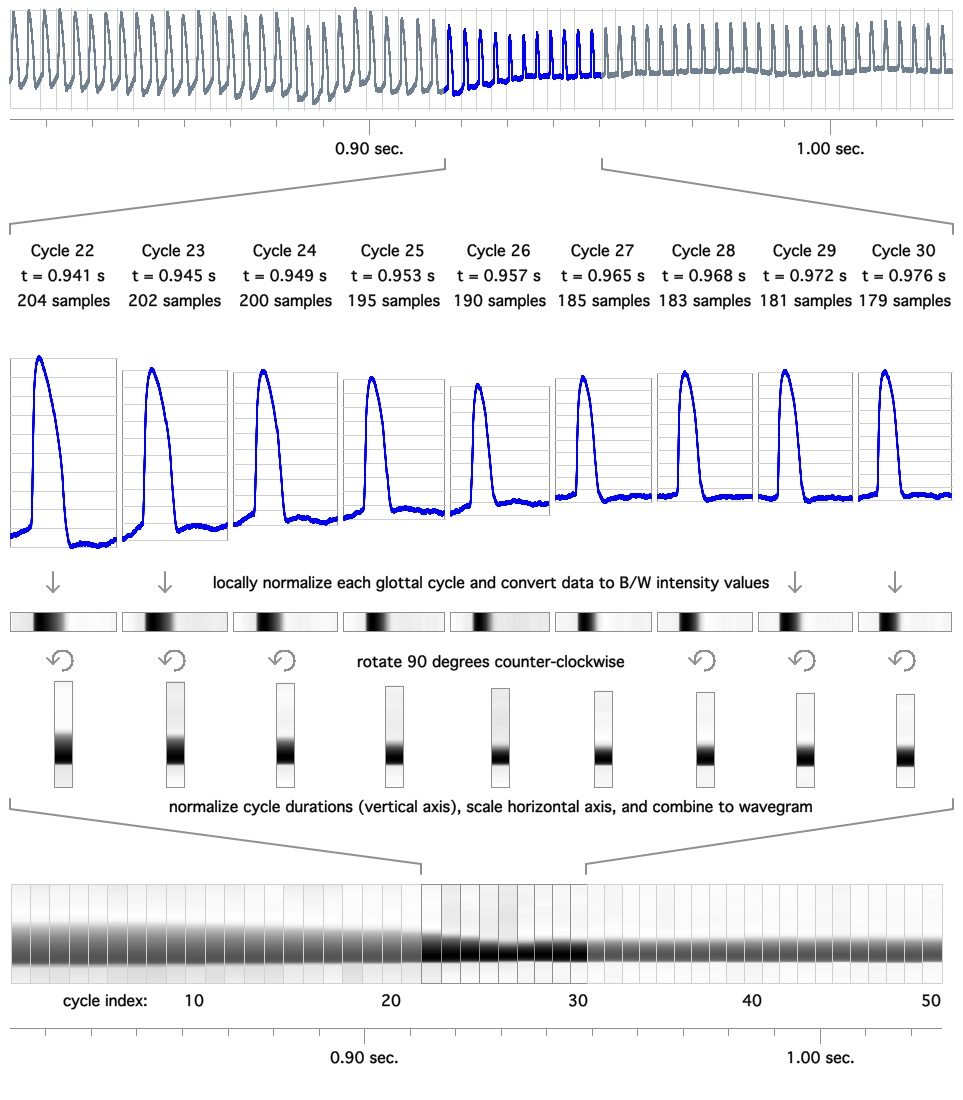
\includegraphics{./img/wavegram.png}
  \caption{The wavegram. Created by Christian T. Herbst under a CC BY-SA 3.0 license.}
  \label{f:wavegram}
\end{figure}

A possible limitation of the wavegram method is that it is intended for
a qualitative analysis based on visual inspection. However, wavegram
data can be modelled using generalised additive models (GAMs,
\citealt{hastie1986, zuur2012, wood2017}). GAMs are a family of
generalised models which can fit non-linear effects by additive
combinations of smoothing splines. The flexibility of GAMs allows
researchers to generate a fitted wavegram based on data from multiple
repetitions of a single speaker and from multiple speakers. Random
effects can also be included to account for idiosyncratic differences.
Moreover, the potential for overfitting is reduced by a smoothing
penalty parameter, which constraints the maximum number of basis
functions used to construct the smoothing splines. This paper introduces
wavegram GAMs as a way to quantitatively assess wavegram data. First,
results from a pilot study which informally evaluates the proposed
method are presented (\Cref{s:pilot}). \Cref{s:voicing} illustrates how
to conduct a wavegram GAM analysis of dEGG data through a practical
example in which the wavegrams of vowels followed by voiceless and
voiced stops are compared. Finally, \Cref{s:conclusion} concludes and
discusses limitations of the current implementation of the method and
future directions.

\hypertarget{pilot-study}{%
\section{Pilot study}\label{pilot-study}}

\label{s:pilot}

Synchronised audio and EGG data were obtained from 5 trained
phoneticians, who were asked to produce sustained tokens of /a/ with
modal and breathy voice. The data was collected using a Glottal
Enterprises EG2-PCX2 electroglottograph and a Movo LV4-O2 Lavalier
microphone, at a sample rate of 44100 Hz (16-bit). The acquisition of
the signals was controlled with Audacity running on a MacBook Pro
(Retina, 13-inch, Mid 2014). The placement of the electrodes strap was
checked with the height indicator on the EGG unit. Each participant
uttered 10 consecutive tokens of a sustained /a/ in modal voice,
followed by 10 tokens of a sustained breathy /a/. All subsequent data
processing was performed in Praat \citep{boersma2018}. The onset and
offset of each token were detected with an automatic procedure which
finds voiced and unvoiced intervals (\texttt{To\ TextGrid\ (vuv)}). The
dEGG wavegram data was extracted from the first 8 glottal cycles of a
500 ms window, centred around the mid-point of each token. A glottal
cycle was arbitrarily defined as the interval between two consecutive
EGG minima (see \citealt{herbst2010} for an alternative algorithm). From
each glottal cycle, the relative amplitude of the dEGG signal was
extracted every 10 samples.

A generalised additive mixed model (GAMM) was fitted to the data to
statistically assess differences in vocal fold activity between modal
and breathy voicing (see \citealt{soskuthy2017} and
\citealt{wieling2018} for a practical introduction to fitting GAMs in
R). The following terms were included: the amplitude of the dEGG signal
as the outcome variable, an interaction factor with language and
phonation as a parametric term, a smooth over the glottal cycle index to
model average changes of the dEGG signal across glottal cycles, and a
smooth over the normalised time of the sample within the glottal cycle
(as the proportion of the time relative to the duration of the glottal
cycle) to model average changes of the dEGG signal within the glottal
cycle; two difference smooths over normalised time of the glottal cycle
onset and normalised sample time using a by-variable with the
language/phonation factor; a tensor product interaction between
normalised cycle time and normalised sample time to model changes of
glottal activity through time, and the same tensor product interaction
with a language/phonation by-variable to model phonation-driven
differences in changes of glottal activity. Finally, inter-speaker
differences were modelled with a by-speaker factor smooth over
normalised cycle time. A first-order autoregressive (AR1) model was
included to deal with the relatively high auto-correlation in the
residuals.

\Cref{f:surface-p} shows the modelled wavegrams of modal and breathy
tokens. Since the tokens were produced with sustained phonation, no
appreciable change within each wavegram can be observed. However, the
comparison of the wavegram of modal voice with that of breathy voice
reveals differences between the two phonation types. As a general trend,
the dEGG maximum and dEGG minimum are achieved later within the glottal
cycle in breathy voicing relative to modal voicing. Moreover,
differences in velocity of closing and opening movements of the vocal
folds are signalled by the relative widths of the purple-coloured bands
(around the dEGG maximum) and the green-coloured bands (around the dEGG
minimum). While in modal voicing the green band is wider, the purple
band is in breathy voicing, indicating that the velocity into and out of
the beginning of the closed phase is slower in breathy voicing.
According to the approximate significance of the smooth terms, phonation
has an effect on the shape of the wavegram as expected (\emph{F}(14.681)
= 3.187, Ref.EDF = 19.027, \emph{p} \textless{} 0.001).

\begin{figure}
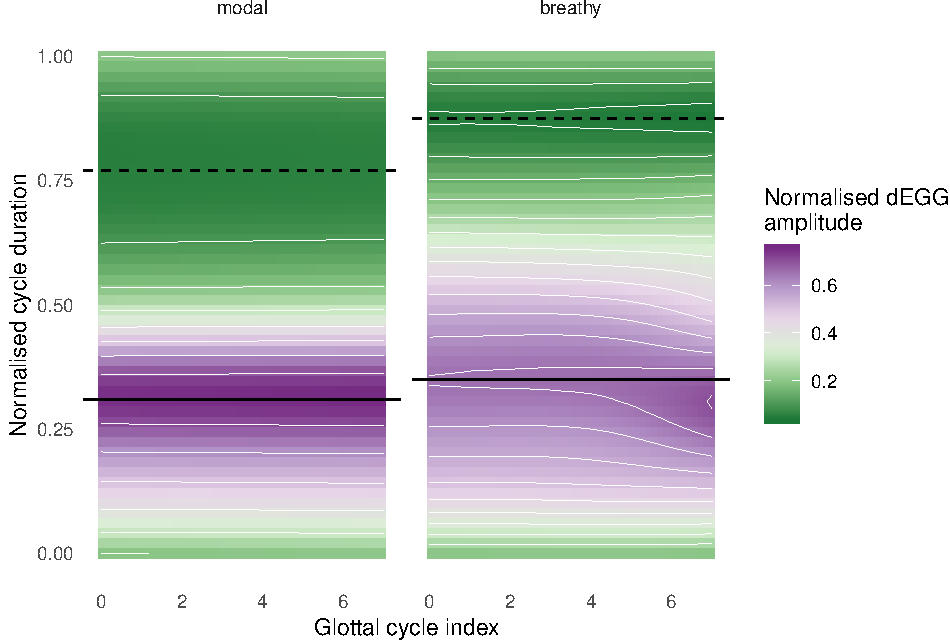
\includegraphics[width=\linewidth]{2019-wavegram_files/figure-latex/surface-p-1} \caption{Fitted wavegram of modal and breathy phonation (Section 2). The horizontal lines represent the dEGG maximum (solid line) and minimum (dashed line).}\label{f:surface-p}
\end{figure}

\hypertarget{wavegram-gam-analysis-of-vowels-followed-by-voiceless-vs.-voiced-stops}{%
\section{Wavegram GAM analysis of vowels followed by voiceless
vs.~voiced
stops}\label{wavegram-gam-analysis-of-vowels-followed-by-voiceless-vs.-voiced-stops}}

\label{s:voicing}

This section further illustrates the use of wavegram GAMs by discussing
a dynamic analysis of changes in vocal folds activity during the
production of vowels followed by voiceless vs.~voiced stops in Italian
and Polish. EGG data was obtained from 9 Italian speakers and 6 Polish
speakers. A detailed description of the experimental materials and
procedures is given in \citet{coretta2018j}. Trochaic words with the
form
C\textsubscript{1}V\textsubscript{1}C\textsubscript{2}V\textsubscript{2}
were used, where C\textsubscript{1} = /p/, V\textsubscript{1} = /a, o,
u/, C\textsubscript{2} = /t, d, k, g/, and V\textsubscript{2} =
V\textsubscript{1} (e.g.~/pata/, /pada/, /poto/, etc.). Processing and
analysis of the EGG data were the same as with the pilot study
(\Cref{s:pilot}), with the exception that data was extracted from every
glottal cycle within the whole duration of the first vowel of the word
stimuli. The vocalic onset and offset were identified as the appearance
and disappearance of higher formant structure respectively
\citep{machac2009}. Vowel duration was then normalised between 0 and 1
for analysis.

\begin{figure}
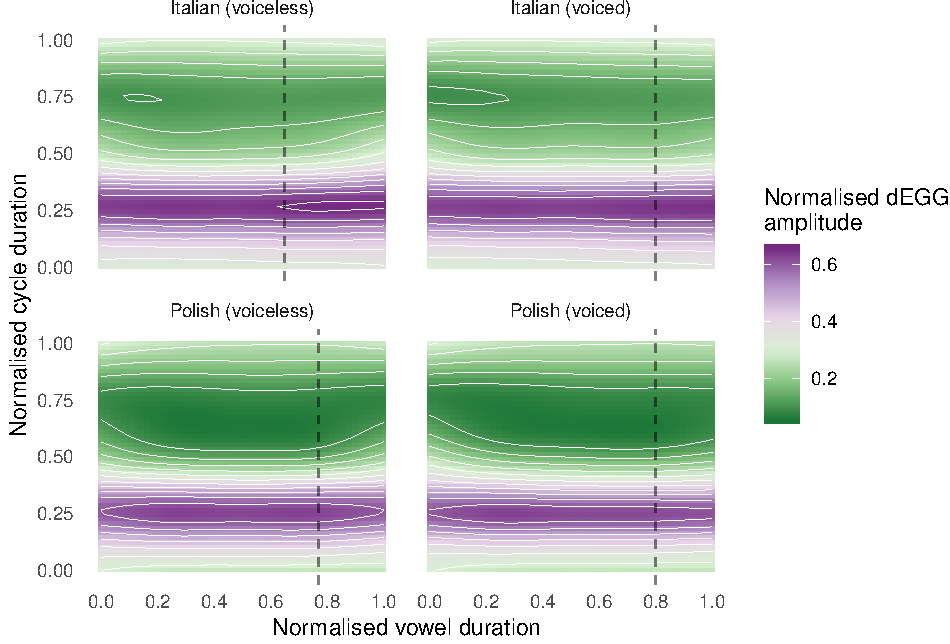
\includegraphics[width=\linewidth]{2019-wavegram_files/figure-latex/surface-1} \caption{Fitted wavegram of vowels followed by voiceless and voiced stops in Italian and Polish (Section 3).}\label{f:surface}
\end{figure}

The same GAM specification as in the pilot study was used to model
changes in glottal activity. Normalised vowel duration was used instead
of glottal cycle index. \Cref{f:surface} shows the modelled wavegrams of
vowels followed by voiceless (left) and voiced stops (right), in Italian
(top) and Polish (bottom). The pilot study showed that a widening of the
wavegram dEGG maximum band (purple) with concomitant shrinkage of the
dEGG minimum band (green) signals greater glottal opening. The change in
band width corresponds to changes in velocity of the execution of the
contacting and decontacting movements. An interesting aspect of modelled
glottal activity concerns the first half of the vowels. The change in
the wavegram indicates a process of decreasing glottal opening (from a
breathier to a more modal phonation). The greater glottal spread
observed at vowel onset could be related to the residual glottal spread
of the preceding voiceless stop /p/. This means that the phonation at
vowel onset is breathier and becomes more modal during the production of
the vowel, stabilising itself at about 20\% of the vowel duration.

Focusing now on the second half of the vowel, the wavegrams in
\Cref{f:surface} show a pattern that is symmetrical to that observed in
the first half \citep{halle1967a}. Namely, glottal opening increases
towards the end of the vowel. The magnitude and timing of the change,
however, differs in the voiceless and voiced contexts. The change is
greater and is implemented earlier in vowels followed by voiceless stops
(left panels) than those followed by voiced stops (right panels). The
earlier and greater glottal spreading in vowels followed by voiceless
stops could be implemented in anticipation of the open glottis required
in the production of voiceless stops as a mechanism to cease vocal fold
vibration. In the case of voiced stops, \citet{halle1967a} propose that
increased glottal width can facilitate voicing while the oral tract is
constricted (cf.~\citealt{westbury1983}, who claims that decreased
glottal width favours voicing).

The wavegrams of vowels followed by voiceless stops also suggest an
effect of language (the GAM terms with a by-language factor return
\emph{p}-values below 0.001). The change in activity before voiceless
stops is initiated earlier in Italian (at around 65\% into the vowel)
than in Polish (at about 80\%). The approximate time of the change onset
is represented by the vertical dashed lines in \Cref{f:surface}. On the
other hand, activity in vowels followed by voiced stops is similar in
the two languages.

The observed greater increase in glottal opening during the production
of vowels followed by voiceless stops in Italian is compatible with the
reported presence of pre-aspiration (breathy or voiceless) in Italian
(geminate) stops
\citep{ni-chasaide1993, stevens2004, stevens2004a, stevens2010, stevens2010b, stevens2014a}.
Increased glottal spreading during vocal fold vibration can be
interpreted as a precursor of voiceless pre-aspiration. An enough opened
glottis can generate enough glottal airflow so as to equalise
sub-glottal and supra-glottal pressure, at which point vocal fold
vibration cannot be supported any longer
\citep{berg1958, rothenberg1967, ohala2011}. The outcome is voiceless
glottal frication, or, in other words, voiceless pre-aspiration.

The patterns of glottal spreading observed here fit with proposed
mechanisms of emergence and of voiceless pre-aspiration and lack
thereof. Pre-aspiration (whether normative or not), now thought to be
possibly more common than previously foreseen \citep{helgason2002}, is
found in several Nordic languages \citet{helgason1999, helgason2002},
English \citep{gordeeva2007, nance2013, hejna2015a}, and, as mentioned
above, Italian, among others. An interesting question is how glottal
spreading in vowels in the context of voiceless stops can lead to the
emergence of voiceless pre-aspiration in some cases and not in others.

\citep{nichasaide1985} argues that pre-aspiration develops as a means to
enhance discriminability in geminate stops by increasing their overall
duration. Under this account, closure shortening is a later development,
rather than the cause of the emergence of pre-aspiration.
\citet{stevens2014} present further experimental evidence that the
duration of pre-aspiration and that of closure are independent in
Italian. In other words, pre-aspiration and closure shortening are
independent. In agreement with \citeauthor{nichasaide1985}'s hypothesis,
the presence of pre-aspiration increased the total duration of the VC
sequence. Pre-closure glottal spreading can thus lead to the emergence
of voiceless pre-aspiration, which can in turn be enhanced by delaying
the onset of stop closure.

\citet{lisker1974} proposes that the laryngeal gesture of glottal
spreading can determine the onset of the stop closure. While some
varieties of English have been reported to show pre-aspiration, others
lack it. \citeauthor{lisker1974} argues that stop closure in voiceless
stops occurs not long after the spreading gesture is initiated in order
to avoid the emergence of voiceless pre-aspiration. The onset of the
closure would be temporally attracted towards the time of glottal
opening onset. Speculatively, this could be one of the mechanisms
responsible for longer closure durations of voiceless stops relative to
that of voiced stops
\citep{lisker1957, umeda1977, van-summers1987, davis1989, de-jong1991},
other things being equal.

To summarise, glottal spreading, which is a typical feature of the
production of voiceless stops, is initiated during the articulation of
the vowel preceding the stop. If the degree of spreading surpasses a
particular threshold, a percept of breathy phonation can arise. At this
point, two possible scenarios can be envisaged. According to one
pathway, breathiness can lead to voiceless pre-aspiration and
subsequence enhancement by closure shortening. In such case,
pre-aspiration could ultimately develop into normative pre-aspiration
like that found in Icelandic. In the alternative scenario, on the other
hand, pre-aspiration is prevented from arising. This can be achieved by
shifiting the timing of the stop closure towards the onset of the
glottal spreading gesture, while keeping the timing of the latter
unchanged. As a consequence, stop closure duration is increased,
resulting in the know pattern of the differential closure durations of
voiceless vs.~voiced stops.

\hypertarget{conclusion}{%
\section{Conclusion}\label{conclusion}}

\label{s:conclusion}

This paper introduced a method for modelling glottal activity as
obtained from wavegram data \citep{herbst2010} using generalised
additive (mixed) models \citep{hastie1986, zuur2012, wood2017}. A pilot
study of the wavegram GAM method showed that the modelled wavegrams are
affected by the global changes in glottal activity depending on the
phonation mode of voicing. In particular, the ability of the model to
distinguish between modal and breathy voicing was tested, and the
results indicated that breathy voicing corresponds to delayed dEGG
maxima and minima within the glottal cycle and decreased velocities of
the contacting phase (with concomitant increased velocity of the
decontacting phase). Building on the results of the pilot study, a
second study was run to investigate glottal activity in vowels followed
by either a voiceless or a voiced stop in Italian and Polish. The
results suggest a change of glottal activity during the second half of
the vowel in anticipation of the glottal configuration of the following
stop (in accordance with \citealt{halle1967a}). The change corresponds
to increasing glottal width in both contexts. However the increase is
greater and implemented earlier in the voiceless than in the voiced
context.

Moreover, the change in glottal activity in vowels followed by voiceless
stops starts earlier in Italian than in Polish. It was argued that the
earlier and grater increase in glottal width in Italian is compatible
with reports of pre-aspiration in some varieties of the language
\citep{ni-chasaide1993, stevens2014a}. It was further speculated that
once an appreciable degree of glottal spreading is implemented during
the vowel, either spreading can result in voiceless pre-aspiration with
subsequent stop closure shortening, or voiceless pre-aspiration can be
avoided by anticipating oral closure while keeping the glottal gesture
(with the consequence of increased closure duration).

A limitation of the proposed wavegram GAM analysis is that, while the
model can statistically assess global differences in the wavegram, more
localised variation still needs to be assessed qualitatively. For
example, while the modelled wavegrams show differences in timing of
change in glottal activity, there is no straightforward way of obtaining
a unique and robust measure of such timing, and statements about this
differences rely on visual inspection of the modelled wavegram. A
wavegram GAM analysis, however, is still useful in providing a method to
model data from multiple repetitions and multiple speakers in a flexible
way. Future work will have to investigate different phonation types
(like creaky voice) and phonetic contexts. More positive tests should be
conducted to assess the reliability of the method. Finally, ways to
obtain quantitative data on timing and degree of changes in glottal
activity will be necessary to further the applicability of the method.

  \bibliography{linguistics}

\end{document}
